\lhead{\emph{Design}}
\chapter{Design}
This chapter first explains the design methods used and the most important design activities and choices made in the design process. Based on this process the final prototype design is presented at the end of the chapter.

\section{Design model and methods}
In this section the model used for designing the final prototype is presented including the different techniques used throughout the design process.

The related works conducts the foundations for an early first prototype. This prototype will then go through an iterative design process, taking a user centered approach. This will enable specifications to emerge during the process and these learnings and modifications will result in new experiments and prototypes. This iterative design model is illustrated in figure \ref{fig:iterative}.

\begin{figure}[htbp]
	\centering
		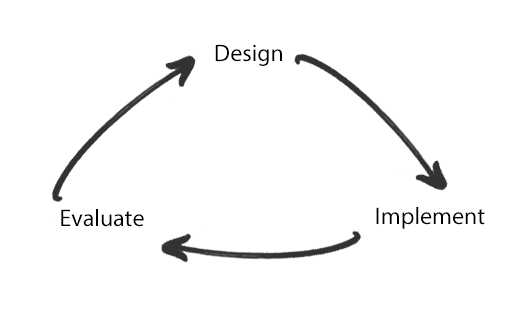
\includegraphics[width=0.6\textwidth,height=\textheight,keepaspectratio]{./Figures/iterative.png}
		\rule{35em}{0.5pt}
	\caption[Iterative Design Model]{Iterative Design Model}
	\label{fig:iterative}
\end{figure}

\subsection{Envisionment}
One of the goals with the final system is that it should be eyes-free i.e. the user should not depend on a visual screen UI at the end. Despite this goal, the use of a screen to visualize e.g. a virtual menu, can be helpful in the design process. This will enable test users to get a quicker and better understanding of how the interaction works. In this design process a mobile device screen will be used for envisionment - this is also called a hifi prototype or software prototype \cite{benyon_designing_2010}.

More concretely track positions, menu depth/state including the users head position and rotation will be mapped visually to a screen dynamically during user interaction. An example of this screen is shown in figure ?

\section{Design process}

\subsection{Head gestures experiment}

\subsection{Sound localization experiment}


\section{Final prototype design}

\subsection{Audio menu structure}

%Several studies show that circular auditory menus are the way to go because of horizontally positioned sounds , HRTF, 3D audio...

%Human head normally can be rotated about 140 degrees for shaking and 100 degrees for nodding \cite{lopresti_neck_2000}.

\subsection{Navigation controls}

% prototyping, iterative design process




% OLD STUFF
%An experimental prototype should be developed and tested. 3 types of menus where a test user should perform head gesture interaction to solve small tasks. User is observed and feedback should be given.

%A final prototype should be designed with knowledge from the experimental evaluation. This prototype will go through a "real life" evaluation. It will be evaluated through several days where the user will use the new head gesture based music application and the traditional music application while biking. Again small task could be performed and it could be tested through the users normal use of his/her music application, ending up in a comparison of the traditional vs the new interaction system.


